\section{Ba đường Conic}

Ba đường Conic bao gồm ellipse, hyperbol và parabol.

\subsection{Ellipse}

\begin{defblock}{Ellipse}

    Đường ellipse là tập hợp các điểm sao cho tổng khoảng cách từ nó tới 2 điểm cố định là 1 hằng số.
\end{defblock}

Nghĩa là, với 2 điểm cố định $F_1, F_2$, tập hợp các điểm $M$ sao cho $M F_1 + M F_2 = 2a$ với $a$ là hằng số tạo thành đường ellipse.

Ở trên hệ tọa độ, nếu ta chọn $F_1$ và $F_2$ nằm trên $Ox$ và đối xứng qua $Oy$, tức là $F_1 = (-c, 0)$ và $F_2 = (c, 0)$, thì các điểm $M = (x, y)$ nằm trên ellipse thỏa

$$MF_1 + MF_2 = \sqrt{(x+c)^2 + y^2} + \sqrt{(x-c)^2 + y^2} = 2a$$

Tương ứng với biển đổi thành phương trình

$$\frac{x^2}{a^2} + \frac{y^2}{a^2 - c^2} = 1$$

Đặt $b^2 = a^2 - c^2$ thì phương trình của ellipse trở thành

$$\frac{x^2}{a^2} + \frac{y^2}{b^2} = 1$$

Phương trình này gọi là \textbf{phương trình chính tắc}.

\begin{figure}[ht]
    \centering
    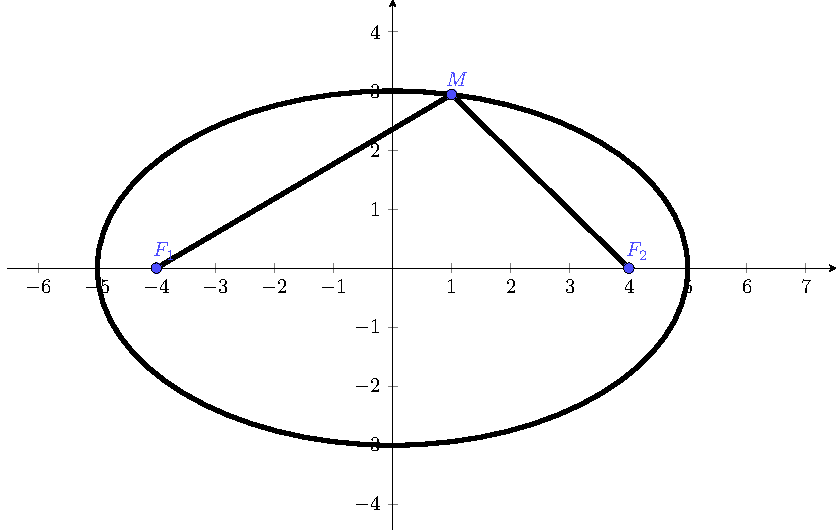
\includegraphics[width=\textwidth]{pics/conics/ellipse.pdf}
    \caption{Ellipse với phương trình $\frac{x^2}{25} + \frac{y^2}{9} = 1$}
\end{figure}

Trong phương trình $$\frac{x^2}{a^2} + \frac{y^2}{b^2} = 1$$

thì $a$ là khoảng cách từ tâm tới 2 biên trái hoặc phải, nên $a$ là \textbf{độ dài bán trục lớn}.

Tương tự, $b$ là \textbf{độ dài bán trục nhỏ} (khoảng cách từ tâm tới 2 biên trên dưới).

Từ cách đặt $b^2 = a^2 - c^2$ tương đương $c^2 = a^2 - b^2$ thì $c$ gọi là \textbf{tiêu cự} của ellipse.

Các điểm $F_1, F_2$ gọi là \textbf{tiêu điểm} của ellipse.

Với ví dụ trên $\frac{x^2}{25} + \frac{y^2}{9} = 1$ thì $a=5, b=3$. Suy ra $c=4$ (lưu ý là $a, b > 0$ và $c \geq 0$).

Các đỉnh nằm ở các tọa độ $(-a, 0), (a, 0), (0, b), (0, -b)$. Các tiêu điểm nằm ở $(-c, 0), (c, 0)$.

\begin{remark}
    Khi $c=0$, tức là 2 tiêu điểm trùng nhau, ta có đường tròn.
\end{remark}

Tâm sai của ellipse là $e = \frac{c}{a} < 1$

\subsection{Hyperbol}

\begin{defblock}{Hyperbol}

    Đường hyperbol là tập hợp các điểm sao cho giá trị tuyết đối hiệu số khoảng cách từ nó tới 2 điểm cố định là 1 hằng số.
\end{defblock}

Nghĩa là, với 2 điểm cố định $F_1, F_2$, tập hợp các điểm $M$ sao cho $| M F_1 - M F_2 | = 2a$ với $a$ là hằng số tạo thành đường hyperbol.

Ở trên hệ tọa độ, nếu ta chọn $F_1$ và $F_2$ nằm trên $Ox$ và đối xứng qua $Oy$, tức là $F_1 = (-c, 0)$ và $F_2 = (c, 0)$, thì các điểm $M = (x, y)$ nằm trên hyperbol thỏa

$$| MF_1 - MF_2 | = | \sqrt{(x+c)^2 + y^2} - \sqrt{(x-c)^2 + y^2} | = 2a$$

Tương ứng với biển đổi thành phương trình

$$\frac{x^2}{a^2} - \frac{y^2}{a^2 - c^2} = 1$$

Đặt $b^2 = a^2 - c^2$ thì phương trình của hyperbol trở thành

$$\frac{x^2}{a^2} - \frac{y^2}{b^2} = 1$$

Đường hyperbol cắt trục $Ox$ tại 2 điểm $A_1 = (-a, 0)$ và $A_2 = (a, 0)$.

Tiêu điểm của hyperbol ở $F_1 = (-c, 0)$ và $F_2 = (c, 0)$.

Đường hyperbol có 2 tiệm cận là đường thẳng $y = \frac{b}{a} x$ và $y = -\frac{b}{a} x$.

Tâm sai của hyperbol là $e = \frac{c}{a} > 1$.

\subsection{Parabol}

\begin{defblock}{Parabol}

    Đường parabol là tập hợp các điểm cách đều một điểm cố định và một đường thẳng cố định.

\end{defblock}

Nghĩa là, với 1 điểm cố định $F$ và đường thẳng cố định $(d)$, parabol là tập hợp các điểm $M$ sao cho $MF = d(M, d)$ với $d(M, d)$ là khoảng cách từ $M$ tới đường thẳng $(d)$.

Phép dời tọa độ cho phép ta dời một hình parabol có đỉnh ở bất kì điểm nào về gốc tọa độ.

Tức là, không mất tính tổng quát, ta chỉ cần xét các parabol dạng $y=ax^2$ là đủ.

Điểm cố định ở trên được gọi là \textbf{tiêu điểm}. Đường thẳng cố định ở trên gọi là \textbf{đường chuẩn}.

Parabol có tính đối xứng nên tiêu điểm nằm trên $Oy$. Đặt tọa độ của nó là $F = (0, f)$.

Đường chuẩn nằm ngang nên ta có parabol là các điểm $M = (x, y)$ sao cho

$MF = \sqrt{x^2 + (y-f)^2}$ và $d(M, d) = y+f$ 
(trường hợp $M$ trùng với đỉnh nên điều kiện của parabol xảy ra tương đương với $M$ cách đều tiêu điểm và đường chuẩn, nghĩa là đường chuẩn có dạng $y=-f$).

Do đó $\sqrt{x^2 + (y-f)^2} = y + f$. Bình phương và biến đổi ta thu gọn được
$$f = \frac{1}{4a}$$

Thường thì ta đặt $p = f$, khi đó phương trình parabol trở thành 
$$x^2 = 4py$$

Đây là dạng chính tắc của parabol với trục đối xứng dọc.

Tâm sai của hyperbol là $e = \frac{c}{a} = 1$.
\newpage